%!TEX root = main.tex

\newpage
\section{Задание}

Синтезировать 4-разрядный ОА, реализующий две операции --- арифметическую и логическую, в соответствии с заданным вариантом (Таблица \ref{table:task}). Работу ОА промоделировать, используя САПР <<Альтера>> Max+plus II.

\begin{table}[H]
	\centering
	\caption{Операции, реализуемые ОА}
	\label{table:task}
	\begin{tabular}{| l | l | l | p{2.2cm} | p{2.2cm} | c | c | c | c | c |} \hline
		\multirow{2}{2cm}{Вариант} & \multirow{2}{2cm}{Операция} & \multirow{2}{2cm}{Код} & \multirow{2}{2.2cm}{Элементы памяти ОА1} & \multirow{2}{2.2cm}{Элементы памяти ОА2} & \multicolumn{5}{c|}{Признаки} \\ \cline{6-10}
		& & & & & S & Z & C' & P & C \\ \hline 
		\multirow{2}{2cm}{2в, 1} & $A \leftarrow A - 1$ & 8421+3 & JK & \multirow{2}{2.2cm}{DC} & + & + & + & + & - \\ \cline{2-4} \cline{6-10}

		& $A \leftarrow A \& B$ & двоичный & JK & & + & + & 0 & + & 0 \\ \hline 
	\end{tabular}
\end{table}


\newpage
\section{Структура ОА}

На этапе структурного синтеза ОА представляют в виде двух частей --- памяти и комбинационной схемы КС (Рисунок \ref{figure:oooa}). КС служит для преобразования входных сигналов Х и информации о состоянии устройства (А) в выходные сигналы Y и сигналы возбуждения элементов памяти U.

\begin{figure}[H]
	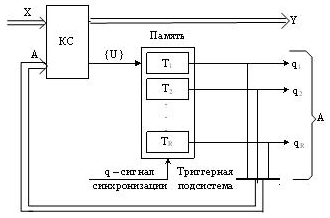
\includegraphics[scale=0.6]{images/2.png}
	\caption{Обобщенная структура ОА}
	\label{figure:oooa}
\end{figure}

Поведение структуры (Рисунок \ref{figure:oooa}) описывается четырьмя группами различных сигналов:

$X$ --- входное слово,

$Y = (X,A)$ --- выходное слово,

$U = \psi(X,A)$ --- слово (функция), обеспечивающее порядок смены состояний автомата

$A$ --- слово, характеризующее состояние автомата.

Внутреннее состояние автомата $А$ определяется состоянием триггеров $a_r \in \{0, 1\}$  и описывается словом состояния $A = (a_1, a_2, a_3, ..., a_i, ... a_r), r = \oline{1,R}$. Множество слов $A$ определяет объем памяти ОА.

Синтезируемый ОА является 4-х разрядным и формирует слово состояния $A = a_3a_2a_1a_0$ .


\newpage
\section{Синтез ОА}

Задача синтеза ОА сводится к:
\begin{itemize}
	\item выбору типа элементов памяти (триггеров), который задан заранее (в данной курсовой работе --- JK-триггеры);
	\item разработке КС, для чего необходимо сформировать систему переключательных функций, описывающую ее поведение:

	$\begin{cases}
			U = \psi(X, A), \\ Y = \lambda(X, A)
	\end{cases}$ (1)
	\item реализации системы ПФ (1) на заданной элементной базе (в данной курсовой работе используется элементная база САПР <<Альтера>> Max+plus II).

\end{itemize}

В случае, если автомат оказывается сложным, задачу синтеза ОА упрощают, декомпозируя (разделяя) его на более простые автоматы ОА$_1$ и ОА$_2$ (Рисунок \ref{figure:decomp}) с одинаковой структурой (Рисунок \ref{figure:srtuct}).

\begin{figure}[H]
	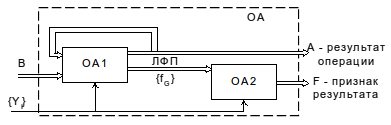
\includegraphics[scale=0.6]{images/3.png}
	\caption{Декомпозиция ОА}
	\label{figure:decomp}
\end{figure}

\begin{figure}[H]
	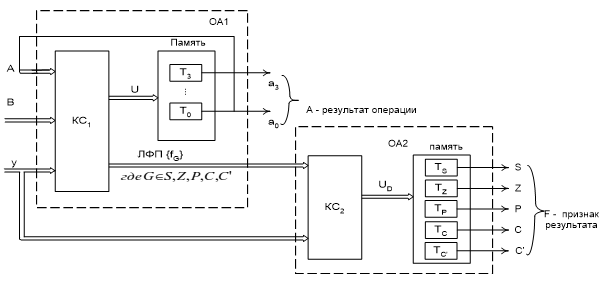
\includegraphics[scale=0.6]{images/4.png}
	\caption{Структурное представление ОА1 и ОА2}
	\label{figure:srtuct}
\end{figure}

Арифметико-логический автомат ОА$_1$ формирует слово результата операции $А$ и сигналы $f_S$, $f_Z$, $f_C'$, $f_P$, $f_C$ --- логические функции признаков (ЛФП), относящиеся к выходным сигналам $Y=\lambda(X, A)$, на основе которых ОА$_2$ формирует уже сами признаки --- слово $F = (S, Z, P, C, C')$ в соответствии с логикой признаков, которая задается таблично (Таблица \ref{table:task}) для каждой отдельной операции.

Операции, реализуемые ОА (Рисунок \ref{figure:decomp}), инициализируются управляющими сигналами $y_i$. В данной работе используется только один управляющий сигнал $y$. Если этот сигнал принимает значение $0$, то выполняется арифметическая операция, иначе --- логическая.

\subsection{Синтез ОА${}_1$}


ОА$_1$ можно рассматривать как многооперационный автомат, способный реализовать не одну, а несколько операций. Синтез автомата ОА$_1$ разделяется на синтез автоматов ОА$^{(0)}_{1}$ и ОА$^{(1)}_{1}$ с памятью на  JK-триггерах, реализующих соответственно: 

\begin{itemize}
	\item операцию декремента $A \leftarrow A-1$ в коде 8421+3, инициируемую сигналом $y_0$.
	\item операцию логического умножения $A \leftarrow A \& B$ , инициируемую сигналом $y_1$.

\end{itemize}

Абстрактное представление ОА$_1$ изображено на рисунке \ref{figure:abs_oa1}.

\begin{figure}[H]
	\begin{subfigure}[b]{0.3\textwidth}
		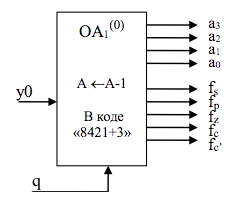
\includegraphics[scale=0.7]{images/abs10.png}
		\caption{ОА$^{(0)}_{1}$}
	\end{subfigure}
	\qquad
	\begin{subfigure}[b]{0.3\textwidth}
		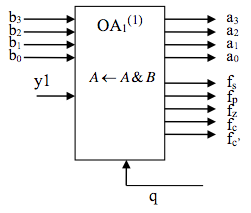
\includegraphics[scale=0.7]{images/abs11.png}
		\caption{ОА$^{(1)}_{1}$}
	\end{subfigure}
	\caption{Абстрактное представление ОА1}
	\label{figure:abs_oa1}
\end{figure}

ОА$^{(0)}_{1}$ реализует операцию над одним словом $А$ с установкой результата, поэтому ОА не декомпозируется, и синтезируется как единый 4-х разрядный ОЭ.

ОА$^{(1)}_{1}$ реализует операцию над двумя 4-х разрядными словами $А$ и $В$ с установкой результата. Сигналы возбуждения и выходов являются функциями восьми аргументов. При рассмотрении такого автомата как единого ОЭ синтез значительно усложнится (КТ будет содержать $256 = 2^8$ наборов), поэтому ОА$^{(1)}_{1}$ декомпозируется и синтезируется как композиция одноразрядных ОЭ.


\subsubsection{Синтез ОА$^{(0)}_{1}$}

Автомат ОА$^{(0)}_{1}$ описывается функциями переходов $A(t+1) = \delta^0(A(t))=\delta^0(a_3,a_2,a_1,a_0)$ и выходов $f^0_{G} = f^0_{G}(A(t)) = f^0_{G}(a_3,a_2,a_1,a_0)$, $G = S, Z, C', P, C$, которые  определяют структуру совмещенной кодированной таблицы (Таблица 2). Каждому значению $A(t)$ ставится в соответствие двоичный вектор следующего состояния автомата $A(t+1) = a^*_3,a^*_2,a^*_1,a^*_0$ как результат функции перехода $\delta^0$ операции $y_0: (A \leftarrow A-1)$.

\begin{landscape}
\begin{table}[H]
	\centering
	\caption{Совмещенная КТ для ОА$^{(0)}_{1}$}
	\label{table:OA10f}
	\begin{tabular}{|l|*{22}{c|}{r|}} \hline
		\multirow{3}{0.5cm}{N}
		& \multicolumn{4}{p{2cm}|}{Текущее состояние ОА$^{(0)}_{1}$}
		& \multicolumn{4}{p{2cm}|}{Следующее состояние ОА$^{(0)}_{1}$}
		& \multicolumn{8}{c|}{ФВ $T^0_j$}
		& \multicolumn{5}{c|}{\multirow{2}{2cm}{ЛФП}} \\ \cline{2-17}

		& \multicolumn{4}{c|}{$A(t)$}
		& \multicolumn{4}{c|}{$A(t+1)$}
		& \multicolumn{2}{c|}{$T_3$} 
		& \multicolumn{2}{c|}{$T_2$} 
		& \multicolumn{2}{c|}{$T_1$} 
		& \multicolumn{2}{c|}{$T_0$}
		& \multicolumn{5}{c|}{} \\  \cline{2-22}

		& $a_3$ & $a_2$ & $a_1$ & $a_0$
		& $a^*_3$ & $a^*_2$ & $a^*_1$ & $a^*_0$
		& $J^{(0)}_{3}$ & $K^{(0)}_{3}$ & $J^{(0)}_{2}$ & $K^{(0)}_{2}$  
		& $J^{(0)}_{1}$ & $K^{(0)}_{1}$ & $J^{(0)}_{0}$ & $K^{(0)}_{0}$
		& $f^{(0)}_{S}$ & $f^{(0)}_{Z}$ & $f^{(0)}_{C'}$ & $f^{(0)}_{P}$ & $f^{(0)}_{C}$ \\ \hline

0 & 	0 & 0 & 1 & 1 & 	1 & 1 & 0 & 0 & 	1 & x & 1 & x & x & 1 & x & 1 & 	1 & 0 & 0 & 1 & 0 \\ \hline
1 & 	1 & 1 & 0 & 0 & 	1 & 0 & 1 & 1 & 	x & 0 & x & 1 & 1 & x & 1 & x & 	1 & 0 & 1 & 0 & 0 \\ \hline
2 & 	1 & 0 & 1 & 1 & 	1 & 0 & 1 & 0 & 	x & 0 & 0 & x & x & 0 & x & 1 & 	1 & 0 & 0 & 1 & 0 \\ \hline
3 & 	1 & 0 & 1 & 0 & 	1 & 0 & 0 & 1 & 	x & 0 & 0 & x & x & 1 & 1 & x & 	1 & 0 & 0 & 1 & 0 \\ \hline
4 & 	1 & 0 & 0 & 1 & 	1 & 0 & 0 & 0 & 	x & 0 & 0 & x & 0 & x & x & 1 & 	1 & 0 & 0 & 0 & 0 \\ \hline
5 & 	1 & 0 & 0 & 0 & 	0 & 1 & 1 & 1 & 	x & 1 & 1 & x & 1 & x & 1 & x & 	0 & 0 & 1 & 0 & 0 \\ \hline
6 & 	0 & 1 & 1 & 1 & 	0 & 1 & 1 & 0 & 	0 & x & x & 0 & x & 0 & x & 1 & 	0 & 0 & 0 & 1 & 0 \\ \hline
7 & 	0 & 1 & 1 & 0 & 	0 & 1 & 0 & 1 & 	0 & x & x & 0 & x & 1 & 1 & x & 	0 & 0 & 0 & 1 & 0 \\ \hline
8 & 	0 & 1 & 0 & 1 & 	0 & 1 & 0 & 0 & 	0 & x & x & 0 & 0 & x & x & 1 & 	0 & 0 & 0 & 0 & 0 \\ \hline
9 & 	0 & 1 & 0 & 0 & 	0 & 0 & 1 & 1 & 	0 & x & x & 1 & 1 & x & 1 & x & 	0 & 1 & 1 & 1 & 0 \\ \hline
		

	\end{tabular}
\end{table}
\end{landscape}

Для каждого из триггеров $T_3 \div T_0$ на основе смены их состояний $a_i \rightarrow a^{*}_i, i=\oline{0,3}$ в соответствии с матрицей переходов (таблица \ref{table:JK_SMW}) формируются двоичные сигналы функций возбуждения (ФВ) $T^0_j, j=\oline{0,3}$, под действием которых они меняют свои состояния. В соответствии с таблицей \ref{table:OA10f} при выполнении операции со словом $A$ устанавливаются логические функции признаков (ЛФП) $f_S$, $f_Z$, $f_P$, $f_C'$. Признак $f_C$ остаётся неизменным.

Признаки:
\begin{itemize}
	\item $f_S$ --- фиксирует знаковый бит результата,
	\item $f_Z$ --- фиксирует нулевой результат,
	\item $f_P$ --- фиксирует четное число единиц результата,
	\item $f_C$ --- фиксирует перенос (заем) из старшего бита результата,
	\item $f_{C'}$---  фиксирует вспомогательный перенос (заем) из бита $а_2$ результата.
\end{itemize}

\begin{table}[H]
	\centering
	\caption{Матрица переходов JK-триггера}
	\label{table:JK_SMW}
	\begin{tabular}{| l | p{1cm} | p{1cm} |} \hline
		\multirow{2}{*}{Переход} & \multicolumn{2}{c|}{Вход триггера}\\ \cline{2-3}
		& J & K \\ \hline
		$0 \rightarrow 0$ & 	$0$ & $x$ \\ \hline
		$0 \rightarrow 1$ & 	$1$ & $x$ \\ \hline
		$1 \rightarrow 0$ & 	$x$ & $1$ \\ \hline
		$1 \rightarrow 1$ & 	$x$ & $0$ \\ \hline
	\end{tabular}
\end{table}

Полученные функции  $J^{(0)}_{3}$, $K^{(0)}_{3}$, $J^{(0)}_{2}$, $K^{(0)}_{2}$, $J^{(0)}_{1}$, $K^{(0)}_{1}$, $J^{(0)}_{0}$, $K^{(0)}_{0}$, $f^{(0)}_{S}$, $f^{(0)}_{Z}$, $f^{(0)}_{C'}$, $f^{(0)}_{P}$, $f^{(0)}_{C}$  заносятся на карты Карно для минимизации (Рисунок \ref{figure:oa10_min_trig}, \ref{figure:oa10_min_flags}).

%!TEX root = main.tex
\kvnoindex
\begin{figure}[H]
	\begin{subfigure}[b]{0.3\textwidth}
	\karnaughmap{4}%
	{$J^{(0)}_3:$}%
	{{$a_1$}{$a_3$}{$a_0$}{$a_2$}}%
	{x0x0xxxxx010xxxx}%
	{%
		\textcolor{Blue}{%
			\put(4, 2){\oval(1.9, 3.9)[l]}
			\put(0, 2){\oval(1.9, 3.9)[r]}
		}%
	}
	\caption{}
	\label{figure:oa10_min_J3}
	\end{subfigure}
	\qquad
	\begin{subfigure}[b]{0.3\textwidth}
	\karnaughmap{4}%
	{$K^{(0)}_3:$}%
	{{$a_1$}{$a_3$}{$a_0$}{$a_2$}}%
	{xxxx100xxxxx0x0x}%
	{%
		\textcolor{Blue}{%
			\put(4, 3.5){\oval(1.9, 0.9)[l]}
			\put(0, 3.5){\oval(1.9, 0.9)[r]}
		}%
	}
	\caption{}
	\label{figure:oa10_min_K3}
	\end{subfigure}

	\begin{subfigure}[b]{0.3\textwidth}
	\karnaughmap{4}%
	{$J^{(0)}_2:$}%
	{{$a_1$}{$a_3$}{$a_0$}{$a_2$}}%
	{xxxx1x0xxx1x0x0x}%
	{%
		\textcolor{Blue}{%
			\put(2, 3.5){\oval(3.9, 0.9)[l]}
			\put(2, 3.5){\oval(3.9, 0.9)[r]}
		}%
		\textcolor{Red}{%
			\put(1, 2){\oval(1.9, 3.9)[t]}
			\put(1, 2){\oval(1.9, 3.9)[b]}
		}%
	}
	\caption{}
	\label{figure:oa10_min_J2}
	\end{subfigure}
	\qquad
	\begin{subfigure}[b]{0.3\textwidth}
	\karnaughmap{4}%
	{$K^{(0)}_2:$}%
	{{$a_1$}{$a_3$}{$a_0$}{$a_2$}}%
	{x1x0x1xxx0x0xxxx}%
	{%
		\textcolor{Blue}{%
			\put(2, 3.5){\oval(3.9, 0.9)[l]}
			\put(2, 3.5){\oval(3.9, 0.9)[r]}
		}%
	}
	\caption{}
	\label{figure:oa10_min_K2}
	\end{subfigure}	

	\begin{subfigure}[b]{0.3\textwidth}
	\karnaughmap{4}%
	{$J^{(0)}_1:$}%
	{{$a_1$}{$a_3$}{$a_0$}{$a_2$}}%
	{x1x0110xxxxxxxxx}%
	{%
		\textcolor{Blue}{%
			\put(2, 0){\oval(3.9, 1.9)[t]}
			\put(2, 4){\oval(3.9, 1.9)[b]}
		}%
	}
	\caption{}
	\label{figure:oa10_min_J1}
	\end{subfigure}
	\qquad
	\begin{subfigure}[b]{0.3\textwidth}
	\karnaughmap{4}%
	{$K^{(0)}_1:$}%
	{{$a_1$}{$a_3$}{$a_0$}{$a_2$}}%
	{xxxxxxxxx1101x0x}%
	{%
		\textcolor{Blue}{%
			\put(2, 0){\oval(3.9, 1.9)[t]}
			\put(2, 4){\oval(3.9, 1.9)[b]}
		}%
		\textcolor{Red}{%
			\put(0.5, 2){\oval(0.9, 3.9)[t]}
			\put(0.5, 2){\oval(0.9, 3.9)[b]}
		}%
	}
	\caption{}
	\label{figure:oa10_min_K1}
	\end{subfigure}

	\begin{subfigure}[b]{0.3\textwidth}
	\karnaughmap{4}%
	{$J^{(0)}_0:$}%
	{{$a_1$}{$a_3$}{$a_0$}{$a_2$}}%
	{x1xx11xxx1xx1xxx}%
	{%
		\textcolor{Blue}{%
			\put(2, 2){\oval(3.9, 3.9)[l]}
			\put(2, 2){\oval(3.9, 3.9)[r]}
		}%
	}
	\caption{}
	\label{figure:oa10_min_J0}
	\end{subfigure}
	\qquad
	\begin{subfigure}[b]{0.3\textwidth}
	\karnaughmap{4}%
	{$K^{(0)}_0:$}%
	{{$a_1$}{$a_3$}{$a_0$}{$a_2$}}%
	{xxx1xx1xxx11xx1x}%
	{%
	{%
		\textcolor{Blue}{%
			\put(2, 2){\oval(3.9, 3.9)[l]}
			\put(2, 2){\oval(3.9, 3.9)[r]}
		}%
	}	
	}
	\caption{}
	\label{figure:oa10_min_K0}
	\end{subfigure}	
	
	\caption{Карты Карно для ФВ ОА$^{(0)}_{1}$}
	\label{figure:oa10_min_trig}
\end{figure}

\begin{figure}[H]
	\begin{subfigure}[b]{0.3\textwidth}
	\karnaughmap{4}%
	{$f^{(0)}_s:$}%
	{{$a_1$}{$a_3$}{$a_0$}{$a_2$}}%
	{x0x0011xx0101x1x}%
	{%
		{%
		\textcolor{Blue}{%
			\put(4, 1){\oval(1.9, 1.9)[l]}
			\put(0, 1){\oval(1.9, 1.9)[r]}
		}%
		\textcolor{Red}{%
			\put(3, 2){\oval(1.9, 1.9)[l]}
			\put(3, 2){\oval(1.9, 1.9)[r]}
		}%
		\textcolor{Green}{%
			\put(2.5, 2){\oval(0.9, 3.9)[t]}
			\put(2.5, 2){\oval(0.9, 3.9)[b]}
		}%
	}
	}
	\caption{}
	\label{figure:oa10_min_fs}
	\end{subfigure}
	\qquad
	\begin{subfigure}[b]{0.3\textwidth}
	\karnaughmap{4}%
	{$f^{(0)}_z:$}%
	{{$a_1$}{$a_3$}{$a_0$}{$a_2$}}%
	{x1x0000xx0000x0x}%
	{%
		{%
		\textcolor{Blue}{%
			\put(1, 3.5){\oval(1.9, 0.9)[l]}
			\put(1, 3.5){\oval(1.9, 0.9)[r]}
		}%
		}
	}
	\caption{}
	\label{figure:oa10_min_fz}
	\end{subfigure}

	\begin{subfigure}[b]{0.3\textwidth}
	\karnaughmap{4}%
	{$f_c:$}%
	{{$a_1$}{$a_3$}{$a_0$}{$a_2$}}%
	{x0x0000xx0100x0x}%
	{%
	\textcolor{Blue}{%
			\put(0.5, 2){\oval(0.9, 3.9)[t]}
			\put(0.5, 2){\oval(0.9, 3.9)[b]}
		}%
	}
	\caption{}
	\label{figure:oa10_min_fc}
	\end{subfigure}
	\qquad
	\begin{subfigure}[b]{0.3\textwidth}
	\karnaughmap{4}%
	{$f^{(0)}_p:$}%
	{{$a_1$}{$a_3$}{$a_0$}{$a_2$}}%
	{x1x0000xx1111x1x}%
	{%
		{%
		\textcolor{Blue}{%
			\put(2, 1){\oval(3.9, 1.9)[l]}
			\put(2, 1){\oval(3.9, 1.9)[r]}
		}%
		\textcolor{Red}{%
			\put(1, 0){\oval(1.9, 1.9)[t]}
			\put(1, 4){\oval(1.9, 1.9)[b]}
		}%
	}
	}
	\caption{}
	\label{figure:oa10_min_fp}
	\end{subfigure}	
	
	\begin{subfigure}[b]{0.3\textwidth}
	\karnaughmap{4}%
	{$f^{(0)}_{c'}:$}%
	{{$a_1$}{$a_3$}{$a_0$}{$a_2$}}%
	{x100110xx0x00x0x}%
	{%
		{%
		\textcolor{Blue}{%
			\put(2, 3.5){\oval(3.9, 0.9)[l]}
			\put(2, 3.5){\oval(3.9, 0.9)[r]}
		}%
	}
	}
	\caption{}
	\label{figure:oa10_min_fc1}
	\end{subfigure}

	\caption{Карты Карно для ЛФП ОА$^{(0)}_{1}$}
	\label{figure:oa10_min_flags}
\end{figure}

В результате минимизации получается система ФВ (2) и ЛФП (3), представленных в МДНФ:

$
\begin{cases}
J^{(0)}_{3} = \oline{a_2}
\\
K^{(0)}_{3} = \oline{a_2} \cdot \oline{a_1} \cdot \oline{a_0}
\\
J^{(0)}_{2} = \oline{a_3} \vee \oline{a_1} \cdot \oline{a_0}
\\
K^{(0)}_{2} = \oline{a_1} \cdot \oline{a_0}
\\
J^{(0)}_{1} = \oline{a_0}
\\
K^{(0)}_{1} = \oline{a_0} \vee \oline{a_3} \cdot \oline{a_2}
\\
J^{(0)}_{0} = 1
\\
K^{(0)}_{0} = 1
\end{cases}
$ (2)

$
\begin{cases}
f^{(0)}_{S} = a_3 \cdot a_2 \vee \oline{a_2} \cdot a_1 \vee a_3 \cdot a_0
\\
f^{(0)}_{Z} = \oline{a_3} \cdot \oline{a_1} \cdot \oline{a_0}
\\
f^{(0)}_{C'} = \oline{a_1} \cdot \oline{a_0}
\\
f^{(0)}_{P} = a_1 \vee \oline{a_3} \cdot \oline{a_0}
\\
f^{(0)}_{C} = 0
\end{cases}
$ (3)


\subsubsection{Синтез ОА$^{(1)}_{1}$}

Автомат ОА$^{(1)}_{1}$ реализует операцию $A \leftarrow A \& B$.

Для упрощения задачи синтеза, декомпозируем автомат ОА$^{(1)}_{1}$ на более простые ОЭ$^{(1)}_i$ (Рисунок \ref{figure:oa11_str}). 

\begin{figure}[H]
	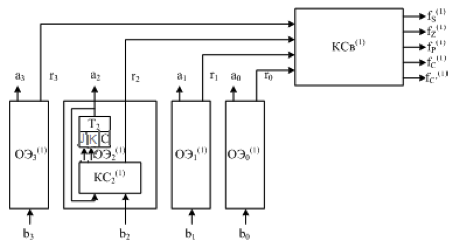
\includegraphics[scale=0.6]{images/oe.png}
	\caption{Структура ОА$^{(1)}_{1}$}
	\label{figure:oa11_str}
\end{figure}

Работа одноразрядного ОЭ$^{(1)}_i$ автомата  ОА$^{(1)}_{1}$ описывается таблицей \ref{table:oe}. Заданные таблично ПФ являются функциями двух аргументов:

$J^{(1)}_i = f(a_i, b_i)$,

$K^{(1)}_i = f(a_i, b_i)$,

$r^{(1)}_i = f(a_i, b_i)$.

Причем $a_i(t+1) = r^{(1)}_i = a_i \& b_i, i=\oline{0,3}$.

\begin{table}[H]
	\centering
	\caption{Описание работы одноразрядного ОЭ$^{(1)}_i$ автомата ОА$^{(1)}_{1}$}
	\label{table:oe}
	\begin{tabular}{| c | c | c | c | c | c |} \hline
		$a_i(t)$ & $b_i(t)$ & $a_i(t+1)$ & $r^{(1)}_i$ & $J^{(1)}_i$ & $K^{(1)}_i$ \\ \hline
		0 & 0 & 	0 & 	0 & 	0 & x \\ \hline
		0 & 1 & 	0 & 	0 & 	0 & x \\ \hline
		1 & 0 & 	0 & 	0 & 	x & 1 \\ \hline
		1 & 1 & 	1 & 	1 & 	x & 0 \\ \hline
	\end{tabular}
\end{table}

Особенностью поразрядного синтеза ОА$^{(1)}_{1}$ является отсутствие информации о состоянии регистра А в целом в момент времени $t$, поэтому ЛФП формируется на основе вспомогательной функции $R$, подаваемой с выходов ОЭ$^{(1)}_i$  (рисунок 4) на входы вспомогательной комбинационной схемы КС$_{(1)}$.

Таблица \ref{table:oa11tab} описывает логику работы КС$_{(1)}$, формирующей сигналы $f^{(1)}_{S}$, $f^{(1)}_{Z}$, $f^{(1)}_{C'}$, $f^{(1)}_{P}$, $f^{(1)}_{C}$. Переключательные функции являются функциями четырех аргументов.

\begin{table}[H]
	\centering
	\caption{Описание принципа установки флагов автомата ОА$^{(1)}_{1}$}
	\label{table:oa11tab}
	\begin{tabular}{|c|*{10}{c|}{r|}} \hline
		\multirow{2}{0.5cm}{N}
		& \multicolumn{4}{p{2cm}|}{$R$}
		& \multicolumn{5}{c|}{ЛФП} \\ \cline{2-10}

		& $r_3$ & $r_2$ & $r_1$ & $r_0$
		& $f^{(1)}_{S}$ & $f^{(1)}_{Z}$ & $f^{(1)}_{P}$ & $f^{(1)}_{C'}$ & $f^{(1)}_{C}$ \\  \hline

0 & 0 & 0 & 0 & 0 & 0 & 1 & 1 & 0 & 0 \\ \hline
1 & 0 & 0 & 0 & 1 & 0 & 0 & 0 & 0 & 0 \\ \hline
2 & 0 & 0 & 1 & 0 & 0 & 0 & 0 & 0 & 0 \\ \hline
3 & 0 & 0 & 1 & 1 & 0 & 0 & 1 & 0 & 0 \\ \hline
4 & 0 & 1 & 0 & 0 & 0 & 0 & 0 & 0 & 0 \\ \hline
5 & 0 & 1 & 0 & 1 & 0 & 0 & 1 & 0 & 0 \\ \hline
6 & 0 & 1 & 1 & 0 & 0 & 0 & 1 & 0 & 0 \\ \hline
7 & 0 & 1 & 1 & 1 & 0 & 0 & 0 & 0 & 0 \\ \hline
8 & 1 & 0 & 0 & 0 & 1 & 0 & 0 & 0 & 0 \\ \hline
9 & 1 & 0 & 0 & 1 & 1 & 0 & 1 & 0 & 0 \\ \hline
10 & 1 & 0 & 1 & 0 & 1 & 0 & 1 & 0 & 0 \\ \hline
11 & 1 & 0 & 1 & 1 & 1 & 0 & 0 & 0 & 0 \\ \hline
12 & 1 & 1 & 0 & 0 & 1 & 0 & 1 & 0 & 0 \\ \hline
13 & 1 & 1 & 0 & 1 & 1 & 0 & 0 & 0 & 0 \\ \hline
14 & 1 & 1 & 1 & 0 & 1 & 0 & 0 & 0 & 0 \\ \hline
15 & 1 & 1 & 1 & 1 & 1 & 0 & 1 & 0 & 0 \\ \hline

	\end{tabular}
\end{table}

Функции возбуждения JK-триггеров (4) и функции выходов (5) формируются на основании таблиц \ref{table:oe} и \ref{table:oa11tab}.

$
\begin{cases}
J^1_3 = f(a_3, b_3) = 0
\\
K^1_3 = f(a_3, b_3) = a_3 \cdot \oline{b_3}
\\
J^1_2 = f(a_3, b_3) = 0
\\
K^1_2 = f(a_3, b_3) = a_3 \cdot \oline{b_2}
\\
J^1_1 = f(a_3, b_3) = 0
\\
K^1_1 = f(a_3, b_3) = a_3 \cdot \oline{b_1}
\\
J^1_0 = f(a_3, b_3) = 0
\\
K^1_0 = f(a_3, b_3) = a_3 \cdot \oline{b_0}
\end{cases}
$ (4)


$
\begin{cases}
f^{(1)}_{S} = f(r_3, r_2, r_1, r_0) = K^4_8 \vee K^4_9 \vee K^4_10 \vee K^4_11 \vee K^4_12 \vee K^4_13 \vee K^4_14 \vee K^4_15
\\
f^{(1)}_{Z} = f(r_3, r_2, r_1, r_0) = K^4_0
\\
f^{(1)}_{P} = f(r_3, r_2, r_1, r_0) = K^4_0 \vee K^4_3 \vee K^4_5 \vee K^4_6 \vee K^4_9 \vee K^4_10 \vee K^4_12 \vee K^4_15
\\
f^{(1)}_{C'}= 0
\\
f^{(1)}_{C} = 0
\end{cases}
$ (5)

Полученные ПФ заносим на карты Карно (Рисунок \ref{figure:oa11_min_trig}, \ref{figure:oa11_min_flag}.

%!TEX root = main.tex

\begin{figure}[H]
\begin{subfigure}[b]{0.3\textwidth}

	\karnaughmap{2}%
	{$J_i:$}%
	{{$b$}{$a$}}%
	{0x0x}%
	{%
	}
	\caption{}
	\label{oa11_J}
\end{subfigure}
\begin{subfigure}[b]{0.3\textwidth}
	\karnaughmap{2}%
	{$K_i:$}%
	{{$b$}{$a$}}%
	{x1x0}%
	{%
	\textcolor{Blue}{
		\put(1,1.5){\oval(1.9,0.9)[]}}
	}
	\caption{}
	\label{oa11_K}
\end{subfigure}
	\caption{oa11mintrig}
	\label{figure:oa11_min_trig}
\end{figure}


\begin{figure}[H]
	\begin{subfigure}[b]{0.3\textwidth}
	\karnaughmap{4}%
	{$f_s:$}%
	{{$r_1$}{$r_3$}{$r_0$}{$r_2$}}%
	{0000111100001111}%
	{%
		\textcolor{Blue}{%
			\put(3, 2){\oval(1.9, 3.9)[t]}
			\put(3, 2){\oval(1.9, 3.9)[b]}
		}%
	}
	\caption{}
	\label{figure:oa11_min_fs}
	\end{subfigure}
	\qquad
	\begin{subfigure}[b]{0.3\textwidth}
	\karnaughmap{4}%
	{$f_z:$}%
	{{$r_1$}{$r_3$}{$r_0$}{$r_2$}}%
	{1000000000000000}%
	{%
		\textcolor{Blue}{
			\put(0.5,3.5){\oval(0.9,0.9)[]}%
		}%	
	}
	\caption{}
	\label{figure:oa11_min_fz}
	\end{subfigure}

	\begin{subfigure}[b]{0.3\textwidth}
	\karnaughmap{4}%
	{$f_p:$}%
	{{$r_1$}{$r_3$}{$r_0$}{$r_2$}}%
	{1001011001101001}%
	{%
		\textcolor{Blue}{
			\put(0.5,3.5){\oval(0.9,0.9)[]}%
			\put(2.5,3.5){\oval(0.9,0.9)[]}%
			\put(1.5,2.5){\oval(0.9,0.9)[]}%
			\put(3.5,2.5){\oval(0.9,0.9)[]}%
			\put(0.5,1.5){\oval(0.9,0.9)[]}%
			\put(2.5,1.5){\oval(0.9,0.9)[]}%
			\put(1.5,0.5){\oval(0.9,0.9)[]}%
			\put(3.5,0.5){\oval(0.9,0.9)[]}%
		}%	
	}
	\caption{}
	\label{figure:oa11_min_fp}
	\end{subfigure}

	\begin{subfigure}[b]{0.3\textwidth}
	\karnaughmap{4}%
	{$f_c:$}%
	{{$r_1$}{$r_3$}{$r_0$}{$r_2$}}%
	{0000000000000000}%
	{}
	
	\caption{}
	\label{figure:oa11_min_fc}
	\end{subfigure}
	\qquad
	\begin{subfigure}[b]{0.3\textwidth}
	\karnaughmap{4}%
	{$f'_c:$}%
	{{$r_1$}{$r_3$}{$r_0$}{$r_2$}}%
	{0000000000000000}%
	{}


	\caption{}
	\label{figure:oa11_min_fc1}
	\end{subfigure}


	\caption{oa11minflags}
	\label{figure:oa11_min_flag}

\end{figure}

После минимизации ФВ (6) и ЛФП (7) будут иметь вид:

$
\begin{cases}
K^1_3 = f(a_3, b_3) = \oline{b_3}
\\
J^1_2 = f(a_3, b_3) = 0
\\
K^1_2 = f(a_3, b_3) = \oline{b_2}
\\
J^1_1 = f(a_3, b_3) = 0
\\
K^1_1 = f(a_3, b_3) = \oline{b_1}
\\
J^1_0 = f(a_3, b_3) = 0
\\
K^1_0 = f(a_3, b_3) = \oline{b_0}
\end{cases}
$ (6)

$
\begin{cases}
f^{(1)}_{S} = r_3
\\
f^{(1)}_{Z} = \oline{r_3} \cdot \oline{r_2} \cdot \oline{r_1} \cdot \oline{r_0}
\\
f^{(1)}_{P} = \oline{r_3 \oplus r_2 \oplus r_1 \oplus r_0}
\\
f^{(1)}_{C'}= 0
\\
f^{(1)}_{C} = 0
\end{cases}
$ (7)


\subsubsection{Объединенные ФВ И ЛФП ОА${}_1$}

В текущий момент такой автомат может выполнять только одну из заданных операций и состояния его меняются в соответствии с логикой реализуемой операции.

На основании составленных ФВ и ЛФП автоматов ОА$^{(0)}_{1}$ и ОА$^{(1)}_{1}$ составим объединенные ФВ (8) и ЛФП (9):

$
\begin{cases}
J_3 = y_0 J^0_3 \cup y_1 J^1_3 = y_0 (\oline{a_2}) \vee y_1(0)
\\
K_3 = y_0 K^0_3 \cup y_1 K^1_3 = y_0 (\oline{a_2} \cdot \oline{a_1} \cdot \oline{a_0}) \vee y_1(\oline{b_3})
\\
J_2 = y_0 J^0_2 \cup y_1 J^1_2 = y_0 (\oline{a_3} \vee \oline{a_1} \cdot \oline{a_0}) \vee y_1(0)
\\
K_2 = y_0 K^0_2 \cup y_1 K^1_2 = y_0 (\oline{a_1} \cdot \oline{a_0}) \vee y_1(\oline{b_2})
\\
J_1 = y_0 J^0_1 \cup y_1 J^1_1 = y_0 (\oline{a_0}) \vee y_1(0)
\\
K_1 = y_0 K^0_1 \cup y_1 K^1_1 = y_0 (\oline{a_0} \vee \oline{a_3} \cdot \oline{a_2}) \vee y_1(\oline{b_1})
\\
J_0 = y_0 J^0_0 \cup y_1 J^1_0 = y_0 (1) \vee y_1(0)
\\
K_0 = y_0 K^0_0 \cup y_1 K^1_0 = y_0 (1) \vee y_1(\oline{b_0})
\end{cases}
$ (8)

$
\begin{cases}
f_S = y_0 f^0_S \cup y_1 f^1_S = y_0 (a_3 \cdot a_2 \vee \oline{a_2} \cdot a_1 \vee a_3 \cdot a_0) \vee y_1 (r_3)
\\
f_Z = y_0 f^0_Z \cup y_1 f^1_Z = y_0 (\oline{a_3} \cdot \oline{a_1} \cdot \oline{a_0}) \vee y_1 (\oline{r_3} \cdot \oline{r_2} \cdot \oline{r_1} \cdot \oline{r_0})
\\
f_{C'} = y_0 f^0_{C'} \cup y_1 f^1_{C'} = y_0 (\oline{a_1} \cdot \oline{a_0}) \vee y_1 (0)
\\
f_P = y_0 f^0_P \cup y_1 f^1_P = y_0 (a_1 \vee \oline{a_3} \cdot \oline{a_0}) \vee y_1 (\oline{r_3 \oplus r_2 \oplus r_1 \oplus r_0})
\\
f_C = y_0 f^0_C \cup y_1 f^1_C = y_0 (0) \vee y_1 (0)
\end{cases}
$ (9)



\clearpage
\subsection{Синтез ОА${}_2$}

 Автомат ОА2 представляется в виде двух частей --- памяти для хранения признаков $S$, $Z$, $C'$, $P$, $C$ (триггеры $T_S$, $T_Z$, $T_{C'}$, $T_P$, $T_C$) и КС$_2$, реализующей логику установки признаков для заданного набора операций. Входными сигналами для ОА$_2$ являются осведомительные сигналы $f_s$, $f_z$, $f_{c'}$, $f_p$, $f_c$ (ЛФП), полученные с выхода ОА$_{1}$, а также сигнал синхронизации $q$.

Через $G$ обозначен один из признаков $S$, $Z$, $P$, $C'$, $C$  (Рисунок \ref{figure:oa2}).

\begin{figure}[H]
	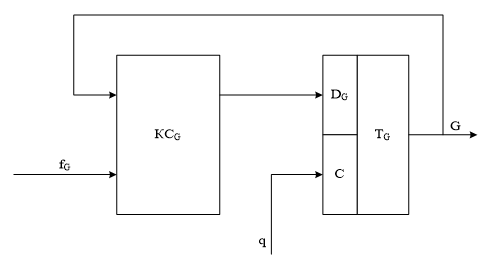
\includegraphics[scale=0.6]{images/oa2.png}
	\caption{Автомат для установки признака G}
	\label{figure:oa2}
\end{figure}

Поскольку признаки $S$, $Z$, $P$, $C'$, $C$ являются независимыми, можно формировать одну таблицу переходов и ФВ для обобщенного признака $G \in \{S, Z, C', P ,C\}$ (Таблица \ref{table:wowmuchlinkswow}). 

Таблица \ref{table:wowmuchlinkswow} делится по строкам на две части. В первой описывается формирование признака $G$ в случае, когда он устанавливается $(*, 0 ,1)$, во второй --- когда не устанавливается ($-$). Следующее состояние $G^*$ триггера признака $T_G$ определяется функциями переходов:
\begin{enumerate}
	\item $G \leftarrow f_G$, если признак устанавливается,
	\item $G \leftarrow G$, если признак не устанавливается.
\end{enumerate}

Сигналы функций возбуждения $D_G$ формируются в соответствии со значением переходов $G^* \leftarrow G$ и матрицей переходов D–триггера (Таблица \ref{table:D_SMW}).

\begin{table}[H]
	\centering
	\caption{Матрица переходов D-триггера}
	\label{table:D_SMW}
	\begin{tabular}{| l | c |} \hline
		Переход & D\\ \hline
		$0 \rightarrow 0$ & 	$0$ \\ \hline
		$0 \rightarrow 1$ & 	$1$\\ \hline
		$1 \rightarrow 0$ & 	$0$ \\ \hline
		$1 \rightarrow 1$ & 	$1$ \\ \hline
	\end{tabular}
\end{table}

\begin{table}[H]
	\centering
	\caption{Таблица переходов и ФВ для признака G}
	\label{table:wowmuchlinkswow}
	\begin{tabular}{| p{2.5cm} | p{2cm} | p{2cm} | p{2cm} | c | p{2.5cm} |} \hline
		\multirow{2}{2cm}{Логика установки признака}
		& Входной сигнал 
		& Текущее состояние $T_G$
		& Следующее состояние $T_G$
		& ФВ
		& \multirow{2}{2cm}{Примечание} \\ \cline{2-5}

		& $f_G$ & $G$ & $G^*$ & $D_G$ & \\ \hline

	   \multirow{4}{2cm}{устанавли-вается} & 0 & 0 & 0 & 0 & \multirow{4}{2cm}{$D_G = f_G$} \\
										   & 0 & 1 & 0 & 0 & \\
										   & 1 & 0 & 1 & 1 & \\
										   & 1 & 1 & 1 & 1 & \\ \hline 
	\multirow{4}{2cm}{не устанавл-ивается} & 0 & 0 & 0 & 0 & \multirow{4}{2cm}{$D_G = G$} \\
										   & 0 & 1 & 1 & 1 & \\
										   & 1 & 0 & 0 & 0 & \\
										   & 1 & 1 & 1 & 1 & \\ \hline 
	\end{tabular}
\end{table}

Подставляя в $D_G$ вместо $G$ конкретные признаки, получают функции возбуждения триггеров признаков $D_S$, $D_Z$, $D_C'$ $D_P$, $D_C$.

\begin{table}[H]
	\centering
	\caption{Объединенные ФВ ОА$_2$}
	\label{table:fvoa2}
	\begin{tabular}{|l|*{11}{c|}{r|}} \hline
		\multirow{2}{*}{Операция} & \multicolumn{5}{c|}{Признаки} & \multicolumn{5}{c|}{ФВ} \\ \cline{2-11}
		& $S$ & $Z$ & $C'$ & $P$ & $C$ & $D_S$ & $D_Z$ & $D_{C'}$ & $D_P$ & $D_C$ \\ \hline
		
		$A \leftarrow A - 1$ & $+$ & $+$ & $+$ & $+$ & $-$ & $f_s$ & $f_z$ & $f_{c'}$ & $f_p$ & $C$ \\ \hline 
		$A \leftarrow A \& B$ & $+$ & $+$ & $0$ & $+$ & $0$ & $f_s$ & $f_z$ & $f_{c'}$ & $f_p$ & $f_c$ \\ \hline 
	\end{tabular}
\end{table}

В соответствии с таблицей \ref{table:fvoa2} сформируем объединенные ФВ для каждого триггера признака:

$D_s = y_0 f_s \cup y_1 f_s$

$D_z = y_0 f_z \cup y_1 f_z$

$D_{c'} = y_0 f_{c'} \cup y_1 f_{c'}$

$D_p = y_0 f_p \cup y_1 f_p$

$D_c = y_0 C \cup y_1 f_c$
